\documentclass[11pt]{article}
\usepackage[utf8]{inputenc}
\usepackage[english, ngerman]{babel}
\usepackage{amsmath,amsthm,verbatim,amssymb,amsfonts,amscd}
\usepackage{enumerate}
\usepackage{listings}
\usepackage{courier}
\usepackage[]{graphicx}
\usepackage[]{epstopdf}
\usepackage[margin=1in]{geometry}
\lstset{
  numbers=left,
  language=C,
  basicstyle=\footnotesize\ttfamily,
  breaklines=true,
  morekeywords={function, NIL}
}
\newcommand{\abs}[1]{\left| #1 \right| }
\setlength{\parindent}{0pt} 

\author{
  Felix Schrader, 3053850 \\ 
  Jens Duffert, 2843110 \\
  Eduard Sauter, 3053470
}
\title{Datenstrukturen und Algorithmen: Haus\"ubung 5}
\begin{document}
\maketitle
\subsection*{Aufgabe 1}
\begin{enumerate}[a)] 
  \item $ $
    \begin{figure}[h!]
      \centering
      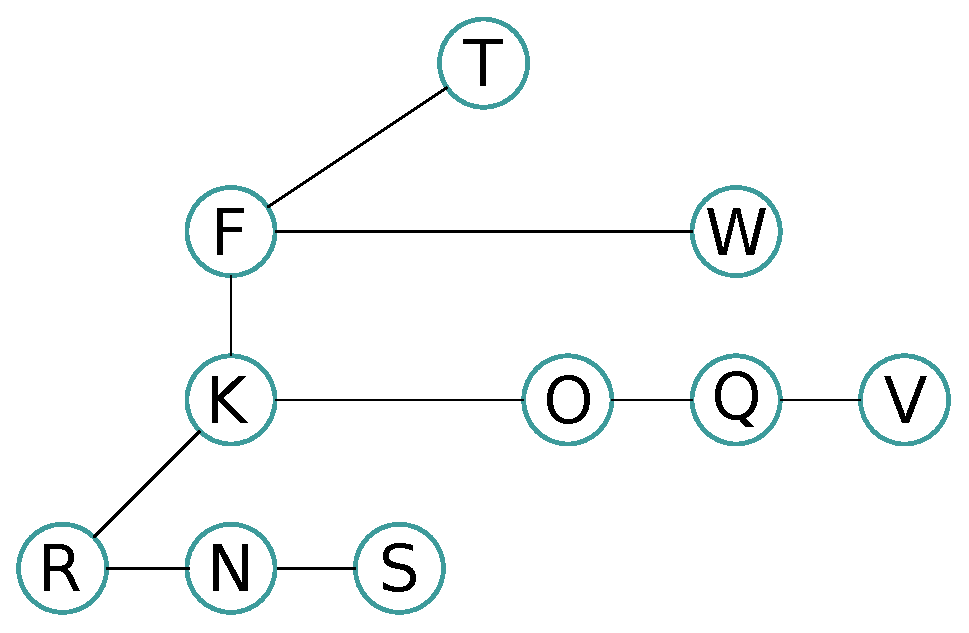
\includegraphics[width=0.4\textwidth]{5_1_a_graph}
      \caption{Binärgraphenkonstruktion nach Vorlesung}
    \end{figure}

    \begin{figure}[h!]
      \centering
      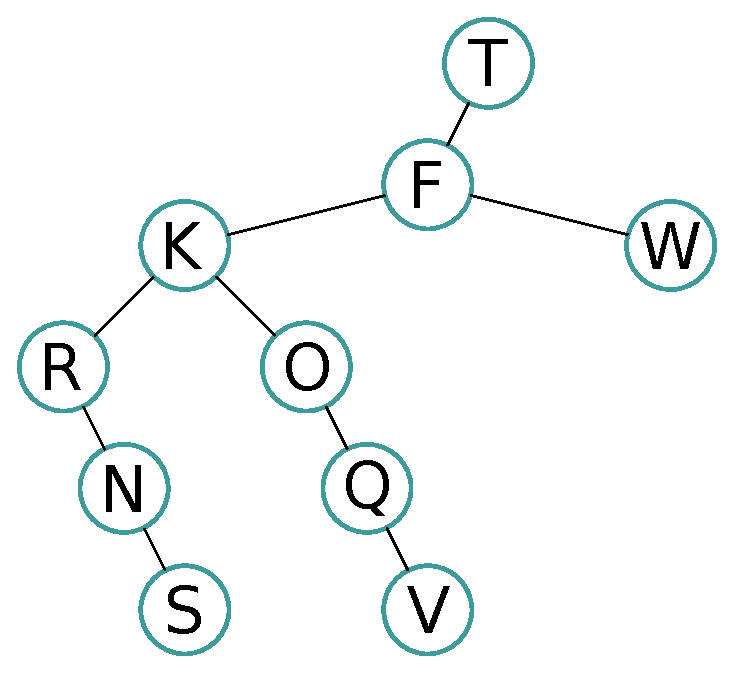
\includegraphics[width=0.4\textwidth]{5_1_a_graph_binary}
      \caption{Binärgraph in kanonischer Darstellung}
    \end{figure}
  \item 
    % Postordnung: links rechts wurzel
    % Präordnung: wurzel links rechts
    % Stufenordnung: nächster nachbar wenn existiert sont erster nachbar
    % auf unterer ebene
    % Symmetrische Ordnung (inorder) links wurzel rechts für binäre bäume
    \begin{description}

      \item[Einfacher Baum] $ $
        \begin{description}

          \item[Stufenordnung] 
            TFWKOQVRNS

          \item[Präordnung]
            TFKRNSWOQV

          \item[Postordnung]
            RNSKFOQVWT

          \item[Symmetrische Ordnung]
            \emph{Ist nur für binäre Bäume definiert}

        \end{description}

      \item[Binärer Baum] $ $
        \begin{description}

          \item[Stufenordnung] 
            TFKWRONQSV

          \item[Präordnung]
            TFKRNSOQVW

          \item[Postordnung]
            SNRVQOKWFT

          \item[Symmetrische Ordnung]
            RNSKOQVFWT

        \end{description}
    \end{description}
    \subsection*{Aufgabe 3}
    \begin{enumerate}[a]
    	
      \item
      Die Idee ist, das für den iterativen Algorithmus ein ADT-Stack erstellt
      wird zuerst. In diesem werden immer die Daten von den einzelnen Punkten
      gespeichert. Nun werden die linken Punkte in diesem Stack schrittweise 
      hinzugefügt. Wenn nun das Ende des Stranges erreicht ist, wird das 
      erste Element aus dem Stack ausgegeben und gelöscht. Dies wird durch den Befehl
      
      
       \lstinputlisting{inorder_tree_walk.js}
          
    \end{enumerate}
     
        
\end{enumerate} 
\end{document}
